\documentclass[12pt]{extarticle}
\usepackage{array}
\usepackage[T1]{fontenc}
\usepackage[Russian]{babel}
\usepackage{booktabs}
\usepackage{graphicx}
\usepackage{spreadtab}
\usepackage{numprint}
\usepackage[margin=3cm]{geometry}
\usepackage{float}
\usepackage{xfp}
\usepackage{amsmath} 
\usepackage{indentfirst}  
\begin{document}
\author{Осипов Александр Б06-604}
\title{Лабораторная работа 1.1.4. ИЗУЧЕНИЕ СТАТИСТИЧЕСКИХ ЗАКОНОМЕРНОСТЕЙ НА 
ПРИМЕРЕ ИЗМЕРЕНИЯ ФОНА КОСМИЧЕСКОГО ИЗЛУЧЕНИЯ}
\maketitle

Работа - https://mipt.ru/upload/Кафедра%20общей%20физики/1/lab/lab_114-2023.pdf

\section{Цель}

На примере статистики регистрации фоновых космических частиц изучить статистические закономерности однородного во времени случайного процесса;
проверить возможность описания исследуемого процесса статистическими законами
Пуассона и Гаусса; измерить среднее число регистрируемых космических лучей в секунду и определить погрешность результата.
\vspace{5mm}

\section{Оборудование}

Счётчик Гейгера—Мюллера, компьютер с интерфейсом для
связи со счётчиком, расчётная программа.
\vspace{5mm}

\section{Теоретическая часть (приницип работаы счётчика)}

Счётчик представляет собой наполненный газом
металлический цилиндр с двумя электродами. Одним из электродов (като-
дом) служит сам корпус. Другим (анодом) является тонкая нить, натянутая
вдоль оси цилиндрического корпуса. Необходимое напряжение (400 В) пода-
ётся на счётчик от смонтированного вместе с ним блока питания через повы-
шающий трансформатор. Радиоактивное излучение (космические частицы)
ионизует молекулы газа, которым наполнен счётчик, а также выбивает элек-
троны из его стенок. Образовавшиеся электроны, двигаясь в сильном элек-
трическом ноле между электродами счётчика, соударяются с молекулами
газа, выбивая из них новые — вторичные электроны. Ускоряясь полем, пер-
вичный и вторичные электроны снова ионизуют газ, и т.д. В результате об-
разуется лавина электронов, и через счётчик протекает кратковременный им-
пульс тока (разряд). Этот импульс и регистрируется электрической цепью
установки, оцифровывается платой аналогово-цифрового преобразователя, и
информация о нём через USB-интерфейс передаётся на компьютер.
\vspace{5mm}

\section{Ход работы}

Измерения проводятся с помощью программы на компьютере.

\begin{enumerate}
    \item В разделе "Эксперимент" запускается эксперимент длительностью 4000с.
    \item В процессе сбора данных программой, выполняется демонстрационное задание:
    \begin{enumerate}
        \item Запускается симуляцию с настройками по умолчанию («Распределение 
Пуассона», интенсивность — 1,0, ускорение — 10). Результаты сохраняются в виде текстовых
и графических файлов.
        \item Симуляция запускается в максимально ускоренном режиме (ускорение = 4000),
изменяя среднюю интенсивность числа частиц.
    \end{enumerate}
    \item Данные обрабатываются в программе, чтобы определить статичестические параметры распределения.
\end{enumerate} 

\section{Обработка результатов}

1. Расчет параметров для разных временных интервалов:

Группировка по 10:

 Среднее <n>: 10.36 

 Стандартное отклонение: 3.075556473070787 

 Погрешность среднего: 0.003844445591338484 

 Интенсивность : 1.036 

 Погрешность интенсивности 0.0003844445591338484

Доля в пределах одной сигма: 68.5% (должно быть ~68.3%)

Доля в пределах двух сигма: 94.75% (должно быть ~95.5%)

Доля в пределах трех сигма: 99.75% (должно быть ~99.7%)

\vspace{5mm}
Группировка по 20:

 Среднее <n>: 20.72 

 Стандартное отклонение: 4.388381187549251 

 Погрешность среднего: 0.010970952968873127 

 Интенсивность : 1.036 

 Погрешность интенсивности 0.0005485476484436563

Доля в пределах одной сигма: 70.0% (должно быть ~68.3%)

Доля в пределах двух сигма: 97.0% (должно быть ~95.5%)

Доля в пределах трех сигма: 100.0% (должно быть ~99.7%)

\vspace{5mm}
Группируем по 40

 Среднее <n>: 41.44 

 Стандартное отклонение: 6.00390445350929 

 Погрешность среднего: 0.03001952226754645 

 Интенсивность : 1.036 

 Погрешность интенсивности 0.0007504880566886613

Доля в пределах одной сигма: 63.0% (должно быть ~68.3%)

Доля в пределах двух сигма: 97.0% (должно быть ~95.5%)

Доля в пределах трех сигма: 100.0% (должно быть ~99.7%)

\vspace{5mm}
Группируем по 80

 Среднее <n>: 82.88 

 Стандартное отклонение: 8.833239634979886 

 Погрешность среднего: 0.08833239634979886 

 Интенсивность : 1.036 

 Погрешность интенсивности 0.0011041549543724858

Доля в пределах одной сигма: 62.0% (должно быть ~68.3%)

Доля в пределах двух сигма: 96.0% (должно быть ~95.5%)

Доля в пределах трех сигма: 100.0% (должно быть ~99.7%)

\newpage
2. Гистограммы распределений (п.15):

\begin{center}
  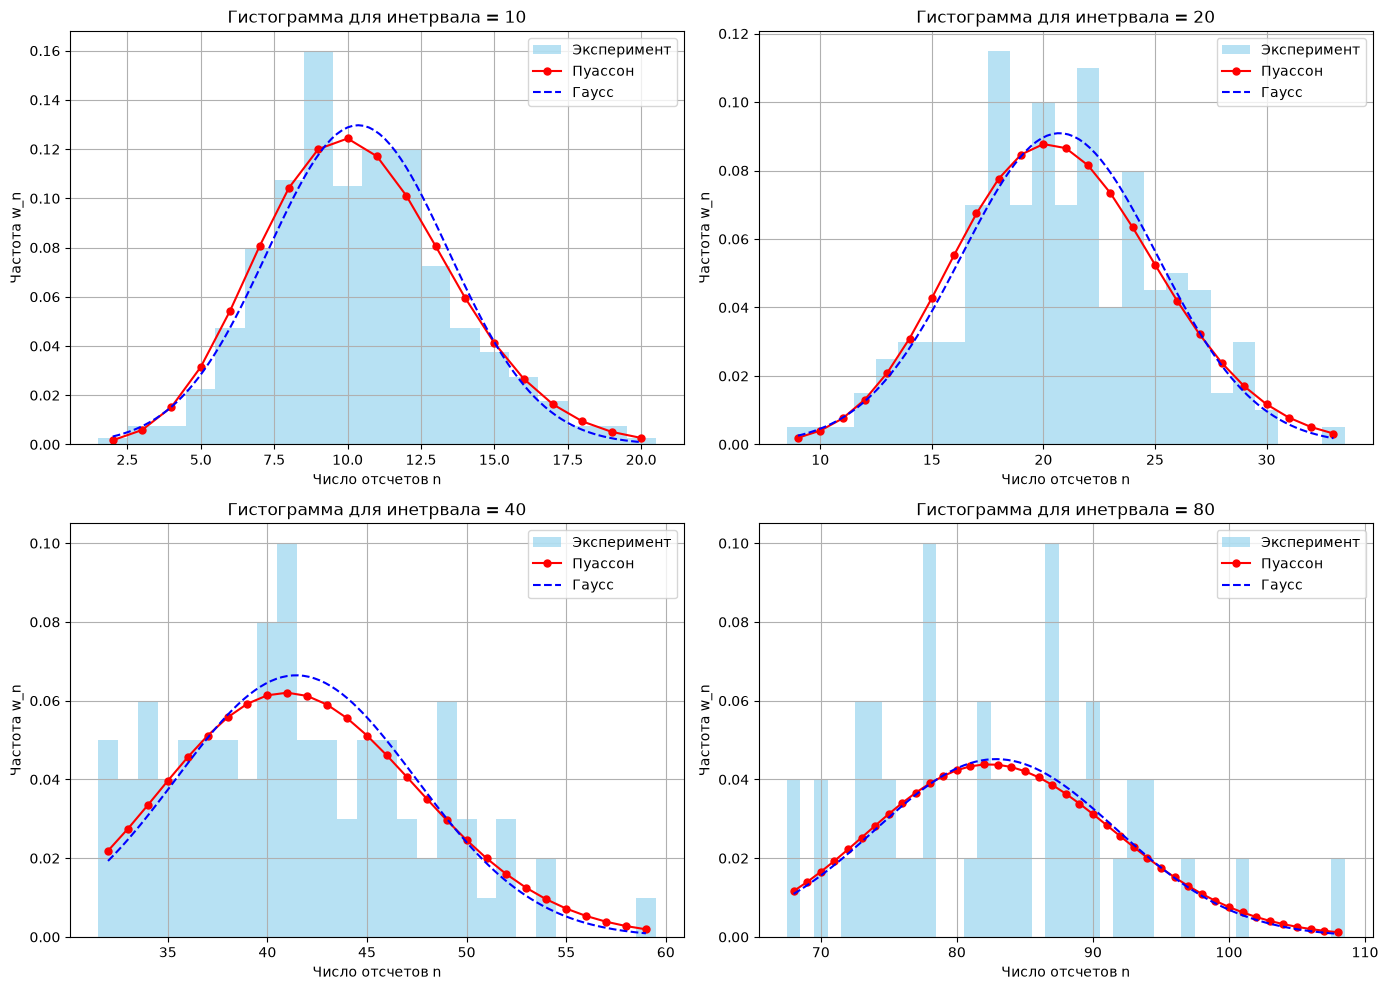
\includegraphics[scale=0.5]{../assets/1.1.4/hist.png}
\end{center}
\vspace{5mm}

\newpage
\textbf{large{Анализ результатов}}

По график и результатам расчета можно увидеть, что наилучшее приближение к графикам
распеределения Пуассона и Гаусса в случае, когда интервал был наименьший. Это связано 
с тем, что при наименьшем интервале мы, фактически, имеем наибольшее количество интервалов:
при разбиении по 10 мы имеем 400 интервалов, при разбиении по 80 мы имеем всего 50 интервалов. 

Согласно ЦПТ, бесконечное количество независимых измерений на графике будет давать 
Гауссовское распределение. В нашем случае это так и получилось: в случае разбиения на интервалы по 10,
мы получили 400 точек, которые на графике близки к Гауссовскому распределению.

Также можно проанализировать, насколько похожи наши распределния на распределение Пуассона.
Пользуясь основным свойством Пуассоновского распределения, сравним среднее и дисперсию:

$\tau = 10$: $\langle n \rangle = 10.36$, $\sigma^2 = 3.075^2 \approx 9.46$

$\tau = 20$: $\langle n \rangle = 20.72$, $\sigma^2 = 4.388^2 \approx 19.25$

$\tau = 40$: $\langle n \rangle = 41.44$, $\sigma^2 = 6.003^2 \approx 36.04$

$\tau = 80$: $\langle n \rangle = 82.88$, $\sigma^2 = 8.833^2 \approx 78.02$

Из результатов видно, что при разбиении на интервалы по 10 наши данные наиболее похожи
на Пуассоновское распределение.

\end{document}
